\begin{figure}
   \begin{subfigure}[t]{0.48\textwidth}
      \begin{nscenter}
         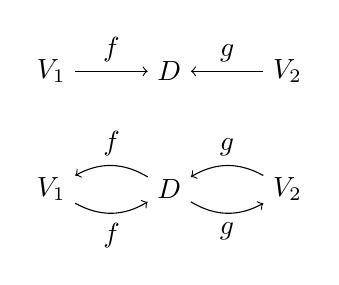
\begin{tikzpicture}[node distance=1.5cm, auto]
            \node (AA) [node distance=2cm] {
               $\Ann{V}_1$
            };
            \node (BB) [right of=AA] {
               $\Ann{D}$
            };
            \node (CC) [right of=BB] {
               $\Ann{V}_2$
            };
            \node (A) [below of=AA] {
               $\Ann{V}_1$
            };
            \node (B) [right of=A] {
               $\Ann{D}$
            };
            \node (C) [right of=B] {
               $\Ann{V}_2$
            };
            \draw[->] (AA) to node {$f$} (BB);
            \draw[->] (CC) to node [swap] {$g$} (BB);

            \draw[->, bend right] (A) to node [swap] {$\lowerAdj{f}$} (B);
            \draw[->, bend right] (B) to node [swap] {$\upperAdj{g}$} (C);
            \draw[->, bend right] (C) to node [swap] {$\lowerAdj{g}$} (B);
            \draw[->, bend right] (B) to node [swap] {$\upperAdj{f}$} (A);
         \end{tikzpicture}
      \end{nscenter}
      \caption{Non-composable Galois connections}
   \end{subfigure}
   \begin{subfigure}[t]{0.48\textwidth}
      \begin{nscenter}
         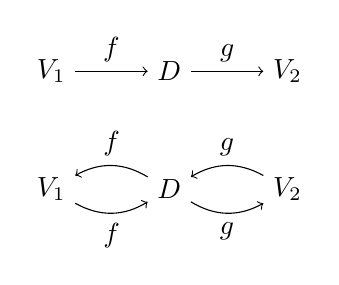
\begin{tikzpicture}[node distance=1.5cm, auto]
            \node (AA) [node distance=2cm] {
               $\Ann{V}_1$
            };
            \node (BB) [right of=AA] {
               $\Ann{D}$
            };
            \node (CC) [right of=BB] {
               $\Ann{V}_2$
            };
            \node (A) [below of=AA] {
               $\Ann{V}_1$
            };
            \node (B) [right of=A] {
               $\Ann{D}$
            };
            \node (C) [right of=B] {
               $\Ann{V}_2$
            };
            \draw[->] (AA) to node {$f$} (BB);
            \draw[->] (BB) to node {$\dual{g}$} (CC);

            \draw[->, bend right] (A) to node [swap] {$\lowerAdj{f}$} (B);
            \draw[->, bend right] (B) to node [swap] {$\dual{\upperAdj{g}}$} (C);
            \draw[->, bend right] (C) to node [swap] {$\dual{\lowerAdj{g}}$} (B);
            \draw[->, bend right] (B) to node [swap] {$\upperAdj{f}$} (A);
         \end{tikzpicture}
   \end{nscenter}
   \caption{Composing via De Morgan duality}
\end{subfigure}
\caption{Galois connections $f$ and $g$ are component-wise composable, but not as Galois connections}
\end{figure}
